\chapter{Design}

Det er i projektet arbejdet lodret ned igennem lagene når der skulle designe nye features. Det er således lavet så der udvikles en feature fuldstændigt ned igennem lagene. Det er derfor valgt at beskrive en feature hele vejen ned igennem for at eksemplificere selve designet af systemmet. For fuld beskrivelse af systemmetdesignet se dokumentationen. 

\section{Modeldesign}

Ud fra domæneanalysen er dataen der giver mening at persistere fundet, og på fig. INDSÆT HER!!!! kan ses hvad der skulle gemmes i forbindelse med barterads.



Som det kan ses på fig gemmes på 
I designet bliver det bestemt hvilke sikkerheder som databasen skal indeholde. Til dette konkrete eksempel kan der en række krav til modellen som skal være opfyldt. Disse ses her:

\begin{itemize}
	\item Barterads skal være tilknyttet en ApplicationUser
	\item Barterads skal have et oprettelsestidspunkt, men dette laves her
	\item Barterads må have en maksiaml beskrivelseslængde på 500 tegn
	\item 
\end{itemize}
Derfor skal der være en måde at tilgå selve databasen og opdatere den. Denne gøres igennem det tidligere nævnte repository pattern. Funktionaliteten til at tilgå databasen er således meget standariseret. 

Men selve funktionaliteten af hvad der sker når klienten skal oprette en barterad, sker igennem serverens controller. 

\section{Controller}  

Som tidligere nævnt tilgår klienten controlleren igennem en URL. Det er sat op på en måde hvor klienten bliver returneret et view til creation af barterads, hvis brugeren er logget ind. Controlleren returnerer login viewet, hvis der ikke er logget ind. Dette bliver gjort igennem controllerend Barterads og aktionen create. Denne controller er således designet til blot at give et view tilbage til brugeren. Når dette view returneres til brugeren er der mulighed for igennem viewet at udfylde elemnterne til en barterad og derefter submitte den. Når denne funktion kaldes tjekkes om de enkelte felter er udfyldt og fortæller brugeren hvis påkrævede fleter mangler, dette gøres vha. asdklaslkd.      

Eksemplificeret gennem en use case f.eks. Create BarterAd

\begin{figure}[H]
	\centering
	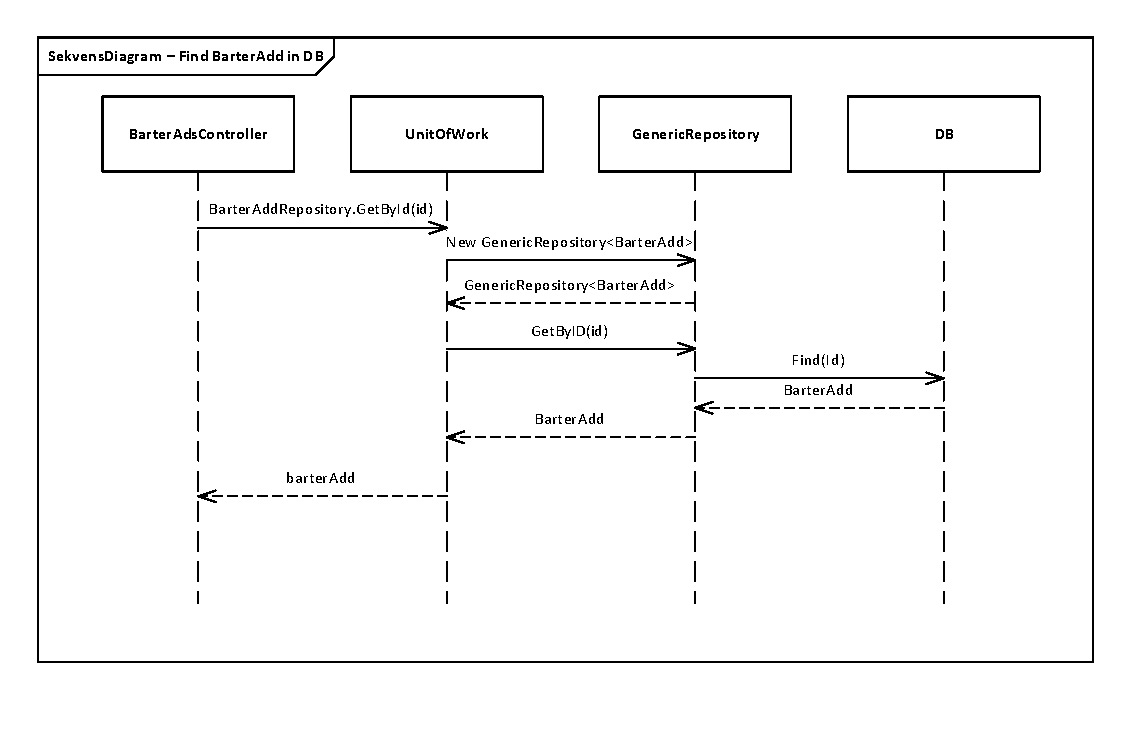
\includegraphics
	[width=140mm]{figures/SDUOFFindBarterAd.PDF}
	\caption{Sekvensdiagram for, hvordan en barterAd bliver fundet i DB}
	\label{fig:UOFFindBarterAd}
\end{figure}

\begin{figure}[H]
	\centering
	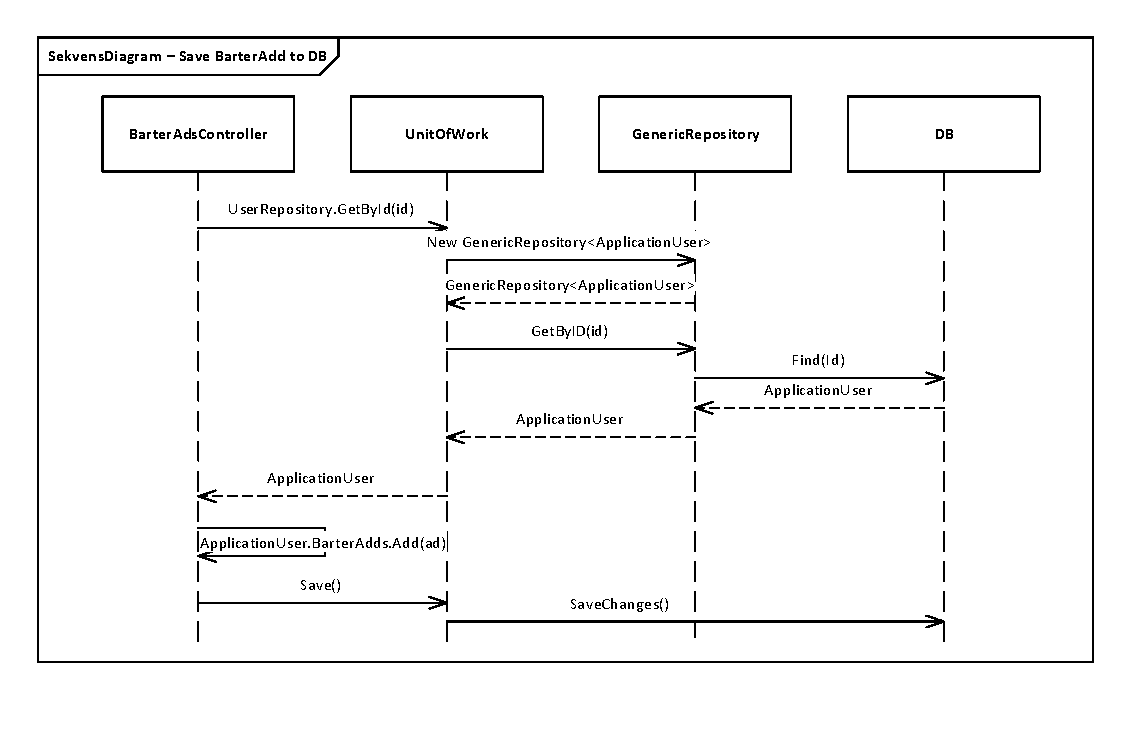
\includegraphics
	[width=140mm]{figures/SDUOFSaveBarterAd.PDF}
	\caption{Sekvensdiagram for, hvordan en barterAd bliver oprettet og gemt i DB}
	\label{fig:UOFSaveBarterAd}
\end{figure}
